\chapter{水下图像合成实验与分析评测}
本章将针对水下图像多模态转译问题设计实验、确定评价指标,验证我们设计的网络模块的有效性,并与基准方法进行对比和分析。

\section{水下图像跨域多模态合成实验设计}
\subsection{实验设置}
基准方法我们总共选取了五种,其中两种经典的图像转译方法CycleGAN~\citep{zhu2017unpaired}和基于分解表示的跨域多模态转译方法MUNIT~\citep{huang2018multimodal},三种最新的图像多模态转译方法DRIT++~\citep{lee2020drit++}、DSMAP~\citep{chang2020domain}和StarGAN v2~\cite{choi2020stargan}。除了不可或缺的经典模型CycleGAN,剩余四种方法都可以完成两个域之间的多模态转译任务。

CycleGAN学习两个域之间的一对一映射,通过循环一致性损失能够很好的学习到目标域的特征;MUNIT, DRIT++ and DSMAP将图像分解为共享的内容空间和不同域的特征空间,然后通过给生成器共享的内容和目标域的特征合成目标域风格相同内容信息的结果;StarGAN v2使用一个生成器结构,通过编码控制生成具有多个特征的多个目标域。所有基准方法的训练代码均来自作者Github提供完成版本。

在我们的实验室中,将$A$域设置为空中域,$B$域设置为多模态水下域,在以上五种基准方法上进行多个数据集的客观实验。在真实水下数据集和合成数据集上设置了针对模糊程度、水颜色、以及特定水质状态的多个实验。

\subsection{数据集设置}
由于水下环境导致采集数据限制,我们的数据集并不是十分充足,因此在一种实验实验设置中用到多个数据集的组合结果。我们在水下图像多模态转译任务中,主要使用到RUIE~\citep{liu2019real}, UWCNN~\citep{li2020underwater}, UVB 2017数据集。EUVP~\citep{islam2019fast}和UIEB~\citep{li2019underwater}数据集就作为补充进行组合实验。其中RUIE,UIEB和EUVP部分数据集是真实世界水下图像结果,UWCNN和UVB 2017是合成图像结果。这些数据集在各个子集数量上并不都是均衡的,所以训练时对模型方法提出了较高的要求。

\begin{figure*}[htp]
    \centering
	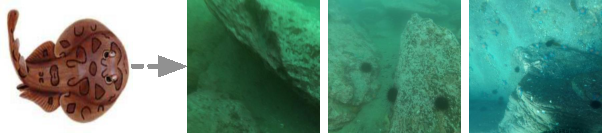
\includegraphics[width=\textwidth]{figures/ruie-dataset.pdf}
	\caption{RUIE数据集多模态转译示例。}
	\label{fig:ruie_dataset}
\end{figure*}

RUIE数据集是一个真实世界获取到的水下不配对图像集。如图~\ref{fig:ruie_dataset}所示,当我们进行水下色偏和清晰度实验训练时,选择RUIE的子集UCCS的300张图片当作水下域,选取EUVP中300张无水子集作为空中域。进行测试实验时,选择EUVP中的100张无水图像作为空中域,测试训练模型,以获得水下多模态域的结果。

\begin{figure*}[htp]
    \centering
	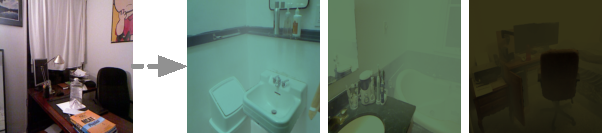
\includegraphics[width=\textwidth]{figures/uwcnn-dataset.pdf}
	\caption{UWCNN数据集多模态转译示例。}
	\label{fig:uwcnn_dataset}
\end{figure*}

UWCNN数据集使用NYU-v2的RGB-D图像来合成深海和近海的十种水类型。基于水下衰减模型,多个衰减系数当作不同的水类型的控制变量。如图~\ref{fig:uwcnn_dataset}所示,当我们进行训练时,选择1200张衰减系数为0即无水域,选择近海type-1,type-3,type-5,type-7作为水下多模态域,每种类型选取300张,这几种水下类型在视觉上有直观可见的区别,方便后续进行定性评价。进行测试时,选择无水域中249张进行测试。

\begin{figure*}[htp]
    \centering
	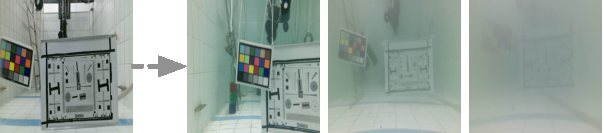
\includegraphics[width=\textwidth]{figures/uvb-dataset.pdf}
	\caption{UVB数据集多模态转译示例。}
	\label{fig:uvb_dataset}
\end{figure*}

Underwater Vision Benchmark 2017 (UVB 2017)是我们实验室用ZED和Kinect立体摄像机捕获的图像和视频数据集。在大连进行了模拟浑浊度实验,将不同浓度的\ce{Al(OH)3}模拟不同水质类型的浑浊度,相机收集相同目标物在不同距离和不同水质下的多种结果。如图~\ref{fig:uvb_dataset}所示训练时,我们选择了66张作为无水域,447张不同深度和浑浊度的结果作为水下多模态域。测试时,无水域选取66张进行测试。

\subsection{评价准则}
为了方便对各个方法进行客观对比,在图像转译角度从转译结果真实性、多样性来进行评价。

\textbf{真实性。}真实性是指给定源域$x_A$图像作为输入,生成的结果应该域目标域$x_B$中的分布尽可能的相同。在我们实验中,生成的水下多模态域的结果应该在质量真实性评价上尽可能的相近。

我们在实验中,真实性指标选取Fréchet Inception Distance(FID)来进行评价。基于Inception score改进,FID最初由Heusel等人~\cite{heusel2017gans}提出。与Inception分数一样,FID分数也使用了Inception v3模型。具体而言,模型的编码层(图像的分类输出之前的最后池化层)被用来抽取输入图像的用计算机视觉技术指定的特征。这些激活函数是针对一组真实图像和生成图像计算的。
使用来自 Inception v3 模型的激活函数输出来归纳每个图像,得分即为Frechet Inception Distance。FID能够完善Inception score没有比较模型生成样本和真实样本统计特性的问题。FID 越低,图像质量越好;反之,得分越高,质量越差,两者关系应该是线性的。较低的FID意味着两个分布之间更接近,也就意味着生成图片的跟真实结果之间相似性较高。

\textbf{多样性。}非成对图像多模态转译问题中,在输入唯一时,能产生目标域的多模态结果。在我们到水下图像多模态转译任务中,在输入一张空中图像时,我们希望能得到多个对应的水下域图像转译结果。即使都是相同的内容,在水质等水下条件不同导致水下图像的模态不一致。对于生成的多种图像,都能跟输入图像拥有相同的内容,再对生成结果进行多样性的评价。

\begin{figure*}[htp]
    \centering
	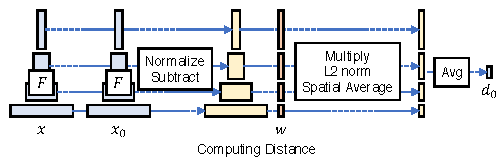
\includegraphics[width=\textwidth]{figures/LPIPS.pdf}
	\caption{}
	\label{fig:lpips}
\end{figure*}

在实验中,我们选用Learned Perceptual Image Patch Similarity (LPIPS)来评价多样性指标。LPIPS最初由Zhang等人~\cite{zhang2018perceptual}提出,用于衡量成对图像之间的相似程度。相比于传统的图像相似度评价指标,LPIPS指标得到的结果和人的视觉评价有更高的相关性。对于多对图像,排列组合成平方次图像对,计算每对之间的相似性,求得平均值作为指标的结果。

\section{水下图像跨域多模态合成结果分析}
\subsection{定性结果分析}

\begin{figure*}[htp]
    \centering
	\includegraphics[width=\textwidth]{figures/RUIE_random_1.pdf}
	\caption{在RUIE数据集上,基准方法和我们提出的方法在目标域随机采样生成的多模态结果比较。}
	\label{fig:ruie_random_1}
\end{figure*}

\begin{figure*}[htp]
    \centering
	\includegraphics[width=\textwidth]{figures/RUIE_random_2.pdf}
	\caption{在RUIE数据集上,基准方法和我们提出的方法在目标域随机采样生成的多模态结果比较。}
	\label{fig:ruie_random_2}
\end{figure*}

图~\ref{fig:ruie_random_1}和图~\ref{fig:ruie_random_2}展示了不同方法在RUIE数据集上的定性结果对比。第一行Real图像表示模型输入图像,之后每行都是对应标记方法获得的结果。从对比图中可以看到,CycleGAN+noise方法的转译结果比较真实,内容信息保留完整,但是噪声被忽略,不同风格采样信息加入的每行之间没有多模态样式的结果;MUNIT方法转译结果质量较差,内容丢失了大量的信息,内容轮廓信息几乎全部丢失,尽管模态之间能看出区别,从行结果上看同样的风格采样信息影响的风格样式并没有一致;DSMAP方法中每行风格信息影响的样式上能看出一致的差异,很明显内容和风格也没有分解彻底,DSMAP的内容收风格样式的影响很严重,在内容细节上没有多少保留,可以看出DSMAP对于内容的处理非常粗糙,生成结果边缘也有伪影的出现。DRIT++方法的结果,内容轮廓能够得到有效的保留,具体内容细节丢失十分严重,DRIT++有多模态效果,但每行模态没有没有实现一致的效果;StarGAN v2方法生成的结果很差,视觉上是学习到了海底样式,但是内容没有有效保留并控制模态样式变化,通过训练没有成功学习到并实现我们想要的多模态转译任务。而本文提出的多模态转译方法,简洁有效的将内容信息和风格信息进行拆分,在内容上,能够极好的保留目标物和水纹理等轮廓和目标颜色变化等细节,在风格上,每行相同风格信息输入能够实现每行风格样式结果的一致,定性视觉上,真实有效地实现水下图像多模态的合成。

\begin{figure*}[htp]
    \centering
	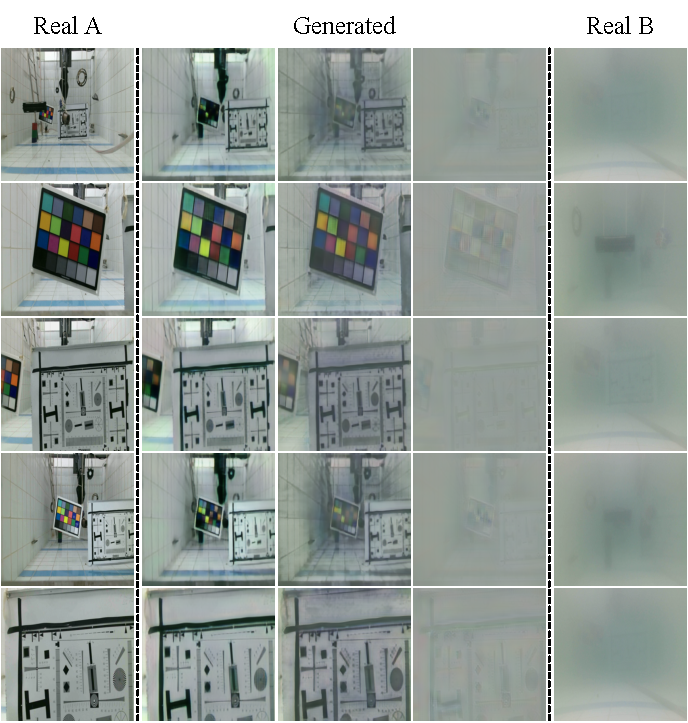
\includegraphics[width=\textwidth]{figures/UVB_random.pdf}
	\caption{在UVB 2017数据集上,基准方法和我们提出的方法在目标域随机采样生成的多模态结果比较。}
	\label{fig:uvb_random}
\end{figure*}

图~\ref{fig:uvb_random}展示了不同方法在UVB 2017数据集上的定性结果对比。第一行Real图像表示模型输入图像,之后每行都是对应标记方法获得的结果。从对比图中可以看到,CycleGAN+noise方法的转译结果较为真实,在浑浊度变化的UVB 2017数据集上尽管内容保持较为完整,像色卡这种比较直观的目标物可以看出转译结果在色卡颜色上保留较好,但是色卡轮廓发生了扭曲,而且没有模态上的变化,噪声对于模态的影响在肉眼上无法辨别;MUNIT方法转译结果内容上可以较好的保留,在目标物轮廓上依旧会发生形变,导致目标物视觉上扭曲,在风格样式上,对于较近的目标物,模糊程度的变化不明显,对于较远的目标物,能够明显看出浑浊程度在不同模态样式上发生了变化,会出现数据集中模糊不存在的绿色雾状效果,越远的位置绿色雾状效果越明显;DSMAP方法转译结果类似MUNIT转译结果,在目标物在内容上会发生形变,在色卡各个颜色之间的扭曲会比MUNIT更明显,整体在内容上不够完整但保留度可以接受,在风格上,一样会出现不存在的绿色雾状效果,呈现近处白色模糊远处绿色模糊的效果;DRIT++方法转译结果,内容上不能保留让人满意的结果,对于内容轮廓能够很好的进行保留,但是对于内容信息,没有得到有效的重视,对于颜色比较复杂的内容部分,直接被黑色阴影填充,导致内容没有完整保留,风格基本上都是水下域中的白色模糊,却会出现棋盘网格样式,是网络结构设计导致的问题;StarGAN v2方法转译结果,在UVB 2017数据集上能有比RUIE真实水下数据集明显成功的转译结果,可以看出StarGAN v2对于数据集本身有一定的要求,在UVB 2017数据集上,内容可以基本保留完整,在色卡上可以看出有轻微的扭曲变形,但是颜色基本保持完整,对于远处的目标物形状基本也完整,风格样式上,视觉效果不明显,多行之间无法清楚辨认出是来自不同模态的结果。而本文提出的水下图像多模态转译方法,内容能够几乎全部被完整保留,不论位置较近还是较远的目标物颜色都没有发生改变仅有模态导致的一定程度模糊、形状也是无扭曲的保留,三个模态的三行结果可以明显看出有样式上的区别,且每个模态影响的风格样式都保持了不同目标上的一致性。可以明显的看出我们的模型在UVB 2017数据集上也可以展现较好的效果。

\begin{figure*}[htp]
    \centering
	\includegraphics[width=\textwidth]{figures/UWCNN_random.pdf}
	\caption{在UWCNN数据集上,基准方法和我们提出的方法在目标域随机采样生成的多模态结果比较。}
	\label{fig:uwcnn_random}
\end{figure*}

图~\ref{fig:uwcnn_random}展示了不同方法在UWCNN数据集上的定性结果对比。第一行Real图像表示模型输入图像,之后每行都是对应标记方法获得的结果。CycleGAN+noise方法的转译结果真实度较高,对于输入图像中的内容保存完好,可以看出生成结果不存在多模态样式,且噪声被模型忽略,无法扰动生成网络从而合成多模态结果;MUNIT在UWCNN数据集上生成的结果较为真实,内容也保存比较完好,但是在生成结果中,色彩较多的部分(如图~\ref{fig:uwcnn_random}MUNIT生成结果中茶几上的部分)会出现转译失败的情况,生成结果能出现多模态效果,每行同一种风格样式编码无法控制模态一致性;在MUNIT方法上进行改进的DSMAP方法转译效果有明显的提升,在内容上基本保留完整,仔细看细节会有轻微的变形,图像中的物体轮廓形状发生了扭曲,对于每行同样的风格编码输入,能有整齐一致的模态变化,在风格上的转译是十分成功地,唯一的缺憾就在于内容没有保持原有的形态;DRIT++方法转译结果,部分内容损失严重,其中轮廓变得模糊,没有清晰的边界,对于雾较为浓厚的模态这种问题不明显,对于雾轻薄的地方,内容的损失就很清晰的展现出来,风格上能有多模态样式,对于每行同一风格编码输入,不能合成一致的模态样式;StarGAN v2结果基本内容能够保存完整,除了内容轮廓有轻微扭曲,整体内容较为完整,且雾与数据集中展示的距离越远的地方雾越厚一致,风格上能生成多模态效果,每行模态效果相似,但不能完全一致,整体风格能看出多模态效果。本文提出的方法在内容上保存完整,无论是内容细节还是内容轮廓都没有发生变化,颜色信息也能在合成过程中保留,对于每行不同的风格编码,每行能有一致的风格样式,且模态间有明显区别的多模态结果。本文提出的方法不仅对于真实水下图像,对于合成水下图像一样能进行有效的多模态控制。


\begin{figure*}[ht]
    \centering
	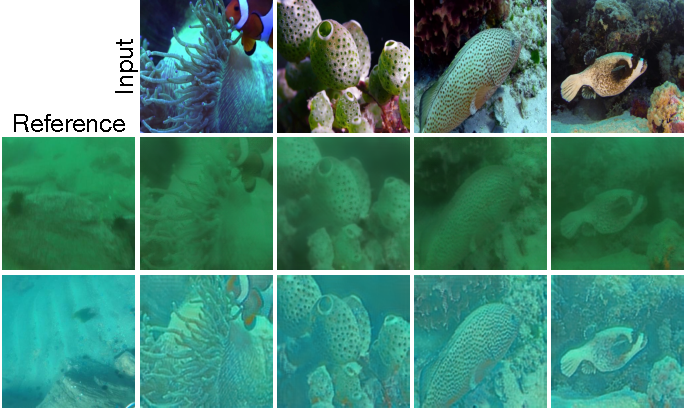
\includegraphics[width=\textwidth]{figures/RUIE_guidance.pdf}
	\caption{RUIE数据集上,本文提出方法用参考图像引导生成指定模态的结果。}
	\label{fig:ruie_guide}
\end{figure*}

图~\ref{fig:ruie_guide}展示了本文提出方法在参考图像引导方式上的多模态结果。对于输入图像,我们给出明确的参考风格图像,将参考图像编码成可以被生成器获取到的风格编码,如此可以合成指定参考风格的合成结果。从每一列可以看出,输入图像的内容得到了很好的保留,细节和轮廓都没有发生任何损失,从每行可以看出,风格影响的水质和模糊程度在不同输入图像上也影响一致。这说明,本文提出的方法能够有效的将图像中的内容和风格进行拆解,内容信息作为恒定不变的部分,在转移过程中需要完整的保留,风格信息作为模态的控制变量,在转译时,源风格信息要彻底清除,且被目标风格替换带入转译过程。

\begin{figure*}[ht]
    \centering
	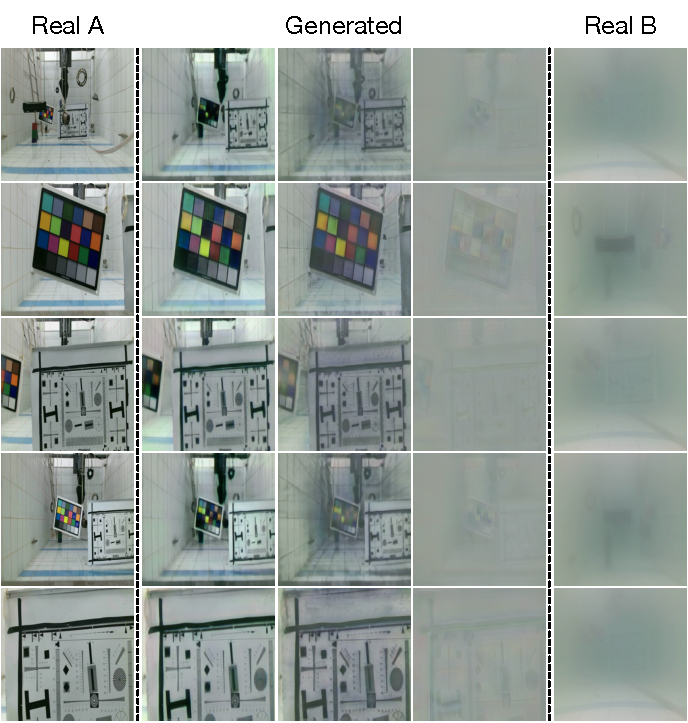
\includegraphics[width=\textwidth]{figures/UVB-change.pdf}
	\caption{在UVB 2017数据集上,浑浊程度样式逐步变化过程。}
	\label{fig:uvb-change}
\end{figure*}

图~\ref{fig:uvb-change}展示了本文提出方法在UVB 2017数据集模态逐步变化过程中的效果。图中Real A代表输入图像,Real B代表目标图像,中间为模态生成结果。我们的方法除了如图~\ref{fig:ruie_guide}中展示的让输入图像A生成目标图像B模态下的结果外,还可以合成逐步从模态A样式变化至模态B样式的结果。A是水下没有浑浊的图像,B是水下浑浊明显的图像,从生成的结果中可以看到,生成图像从左往右依次变化过程中,浑浊度不断增加,趋向于B中浑浊程度。在生成结果中,模态逐步变化,图像中的内容保持不变,仅仅是浑浊程度这个样式上发生了改变,内容的颜色、细节和轮廓都保存完整。

\subsection{定量结果分析}

真实性和多样性定量指标如表~\ref{tab:ruie_comparison}、~\ref{tab:uvb_comparison}和~\ref{tab:uwcnn_comparison}所示。在定量结果分析,我们对比了CycleGAN、MUNIT、DRIT++、DSMAP、StarGAN v2基准方法在RUIE、UVB 2017和UWCNN数据集上的实验评价,所有方法都是用作者Github代码给出的标准测试,采用相同指标的标准评价,下列结果能够客观的进行对比分析。

\begin{table*}[ht]
\centering
\caption{在RUIE数据集上,基准方法和我们方法的真实性和多样性定量比较。}
  \begin{tabular}{c|ccccccccc}
    \hline\noalign{\smallskip}
    方法 & CycleGAN+noise & MUNIT & DRIT++ & DSMAP & StarGAN v2 & Ours \\
    \noalign{\smallskip}\hline\noalign{\smallskip}
    FID$\downarrow$ & 143.4 & 139.4 & 179.2 & 139.6 & 121.1 & \textbf{83.2} \\
    LPIPS$\uparrow$ & 0.534 & 0.452 & 0.575 & 0.513 & 0.431 & \textbf{0.579} \\
    \noalign{\smallskip}\hline
  \end{tabular}
  \label{tab:ruie_comparison}
\end{table*}

从表格~\ref{tab:ruie_comparison}中我们可以看到,在真实水下获取到的RUIE数据集上从空中到水下多模态域转译的定量结果对比。CycleGAN+noise方法评价中,FID指标较高,说明跟真实水下图像差距较大,分析原因主要是因为CycleGAN+noise生成结果较为固定,跟真实多模态样本之间会存在较大的差异,输入图像的合成结果加上噪声也没有多模态样式,但是自身转译结果是真实样本多模态样式中的任意一种,在计算LPIPS指标时,结果看起来令人满意,实际上同一输入无法产生多模态结果;MUNIT方法评价中,FID指标较高,说明跟真实水下图像差距较大,这主要是由于合成结果中内容损失严重,内容在轮廓上都无法与模态样式分离,在计算LPIPS指标时,能生成多模态效果但是模态之间效果差别较小,多样性不够多导致LPIPS指标较低;DRIT++方法评价中,由于合成的结果内容细节信息丢失严重,在与真实样本计算FID指标时,必然会有很巨大的差距,所以FID指标最高,真实性最差,在计算LPIPS指标时,对于不同的风格采样,同一输入可以生成不同模态养的结果,因此多样性足够高,可以看出与我们方法指标相差无几,但是对于每种特定的风格采样,不同输入无法生成一致模态的结果;DSMAP方法是在MUNIT方法上进行改进,将域共享内容信息拆分出域特有内容信息,实际上将内容和风格进一步分解,这样获得到的内容信息更加纯净,在测量指标时,由于合成结果内容损失严重,除了部分轮廓能辨认其余内容信息全部丢失,在计算FID时,跟真实样本结果之间的差异必然巨大,导致FID指标较高,在计算LPIPS指标时,输入每种模态风格能有一致的合成模态结果,因此多样性存在;StarGAN v2方法评价中,由于生成结果内容没有有效保留,但是学习到了海底样式,所以在评价FID指标时,结果稍微有点高,存在多模态效果但是模态之间差异不明显,在评价LPIPS指标时结果较低,多样式不足。本文中提出的方法评价中,生成结果内容保留完好,且合成结果接近真实样本,所以FID结果较低,说明合成结果真实性高;能够通过对目标域风格随机采样或者通过参考图像进行引导合成真实的多模态结果,有足够多的模态样式,所以LPIPS指标最高,说明合成结果多样性充足。

\begin{table*}[ht]
\centering
\caption{在UWCNN数据集上,基准方法和我们方法的真实性和多样性定量比较。}
  \begin{tabular}{c|ccccccccc}
    \hline\noalign{\smallskip}
    方法 & CycleGAN+noise & MUNIT & DRIT++ & DSMAP & StarGAN v2 & Ours \\
    \noalign{\smallskip}\hline\noalign{\smallskip}
    FID$\downarrow$ & \textbf{80.7} & 232.1 & 290.7 & 138.8 & 149.8 & 129.6          \\
    LPIPS$\uparrow$ & 0.490         & 0.647 & 0.668 & 0.513 & 0.595 & \textbf{0.736} \\
    \noalign{\smallskip}\hline
  \end{tabular}
  \label{tab:uwcnn_comparison}
\end{table*}

从表格~\ref{tab:uvb_comparison}中我们可以看到,在合成数据集UWCNN空中到水下多模态图像域转译的定量结果对比。CycleGAN+noise方法测评中,图像真实性非常高,跟数据集中部分模态真实样本分布接近,在计算FID时,CycleGAN+noise和真实数据之间的差距非常小,在计算LPIPS时,由于该方法合成的样本不受风格编码的扰动,合成样本的多样性缺乏,因此LPIPS指标较低;MUNIT方法测评中,图像内容上可以较好的保 留,在目标物轮廓上依旧会发生形变,导致目标物视觉上扭曲,在计算FID时,差异较大,扭曲导致真实性下降,在计算LPIPS时,能看出模态在不同风格编码输入时发生变化,所以LPIPS指标较高,多样性结果存在;DSMAP方法测评中,类似MUNIT会发生形变,且扭曲比MUNIT更严重,所以在计算FID时结果值较高,真实性更低,在计算LPISP时,不同输入之间的多模态样式不明显,导致多样性不足,指标较低;DRIT++方法测评中,由于内容信息中复杂的部分被黑色阴影填充,真实性降低,因此FID指标最高,由于不同的模态样式编码输入可以影响合成不同样式,有多样性结果,因此LPIPS值较高;StarGAN v2在UWCNN数据集上可以合成视觉上真实的结果,与真实样本分布较为接近,因此FID较低,但是在风格上缺乏多模态合成结果,因此LPIPS也比较低。本文提出的方法在合成结果中,内容信息保留完整,在所有基于分解的转译方法中,可以FID最低,且多种样式合成结果都有,多样性足够所以LPIPS可以获得最高值。

\begin{table*}[ht]
\centering
\caption{在UVB数据集上,基准方法和我们方法的真实性和多样性定量比较。}
  \begin{tabular}{c|ccccccccc}
    \hline\noalign{\smallskip}
    方法 & CycleGAN+noise & MUNIT & DRIT++ & DSMAP & StarGAN v2 & Ours \\
    \noalign{\smallskip}\hline\noalign{\smallskip}
    FID$\downarrow$ & \textbf{145.1} & 240.4 & 243.7 & 232.6 & 162.9 & 172.7          \\
    LPIPS$\uparrow$ & 0.358          & 0.486 & 0.474 & 0.444 & 0.358 & \textbf{0.493} \\
    \noalign{\smallskip}\hline
  \end{tabular}
  \label{tab:uvb_comparison}
\end{table*}

从表格~\ref{tab:uwcnn_comparison}中我们可以看到,在合成数据集UWCNN空中到水下多模态图像域转译的定量结果对比。CycleGAN+noise方法测评中,转译结果真实度较高,对于输入图像中的内容保存完好,在计算FID时,能够得到最低值,但是由于CycleGAN+noise生成结果不具有多样性,在计算LPIPS时结果较差;MUNIT生成的结果较为真实,内容也保存比较完好,会出现真实样本中不存在的黄色模态,且颜色较多的部分转译会失败,在计算FID时,与真实结果差别较大,真实性不高,FID值很高,在计算呢LPIPS时会出现多种模态样式,且模态间差别很大,所以LPIPS指标较高;DSMAP在内容上基本保留完,也出现了真实样本中不存在的黄色模态结果,FID指标较高,缺乏真实性,合成结果能在模态上出现多样性且模态内的一致性,LPIPS指标结果较高;DRIT++方法测评中,轮廓模糊,边界不清晰,与真实样本结果区别较大,FID指标最高,真实性最低,尽管模态内结果不一致,担合成结果有明显的模态差异,LPIPS指标较高,具有多样性;StarGAN v2结果基本内容能够保存完整,且合成模态非常近似真实样本,FID指标较低,真实性较高,风格上生成的多模态效果模态内不稳定,LPIPS指标较低,多样性不充足。本文提出方法测评中,内容上保存完整,在其他分解表达方法中可以得到最好的FID结果,真实性较高;真实样本中存在的多种样式合成结果都有,多样性充足所以LPIPS最高。

\subsection{消融实验}

为了验证我们设计网络的有效性,主要对于转译器部分进行模块验证。对于我们提出的内容一致性限制的有效性,我们设计了几种消融实验,一是内容一致性限制在MUNIT、DRIT++经典分解表达方法上的有效性;二是MUGAN模型中内容一致性限制的有效性。



\section{水下图像多样式域合成实验设计}
\subsection{实验设置}

\subsection{数据集设置}

\subsection{评价准则}

\section{水下图像多样式域合成结果分析}
\subsection{定性结果分析}

\subsection{定量结果分析}


\subsection{消融实验}
